\chapter{Elementary Number Theory}

%% BASICS
\section{Basic Properties}
In number theory we deal with the properties of various classes of numbers such as the integers, which is any number that can be written without a fractional or decimal component and is denoted with the the symbol $\mathbb{Z}$. Thus, $-7$, $0$, and $2$ are integers; $1.7$ and $\frac{1}{7}$ are not. Incidentally the Latin word "integer" literally means "untouched", hence "whole". Of particular interests is the set of all positive integers, also known as the natural numbers and symbolized by $\mathbb{N}$. However before we immerse ourself in the exciting properties of natural numbers let us first consider that integers are either $even$ or $odd$, more formally we write: 
\begin{defi}\label{num_def}
The $even$ numbers are the numbers written on the form $2k$ and the $odd$ numbers are the numbers written on the form $2k+1$ where $k$ is any integer.
\end{defi}
some arithmetic can be used to check that this indeed yields the desired numbers:
\[\begin{array}{lcl} 
2 \cdot 0     & = & 0 \\
2 \cdot 0 + 1 & = & 1 \\
2 \cdot 1     & = & 2 \\
2 \cdot 1 + 1 & = & 3 \\
:             &   & :
\end{array}\]

The $odd$ numbers may also be expressed as being either one more than a multiple of $4$ or three more than a multiple of $4$. Symbolically, we can say that they are either of the form $4k + 1$ or of the form $4k  + 3$. Again some examples clarifies the smoke
\[\begin{array}{lcl} 
4 \cdot 0 + 1 & = & 1 \\
4 \cdot 0 + 3 & = & 3 \\
4 \cdot 1 + 1 & = & 5 \\
4 \cdot 1 + 3 & = & 7 \\
:             &   & :
\end{array}\]

incidentally this shows that when we divide a $odd$ number by $4$, we must get a remainder of either $1$ or
$3$ \label{remainder}. Armed with this knowledge we can shine some light on the properties of $odd$ numbers:
\begin{cor}
The square of an $odd$ number is $odd$
\end{cor}
\begin{proof}
Consider, by \ref{num_def}, the algebraic form of the square of an odd number
\[\begin{array} {lcl} 
(2k+1)^2 & = & (2k)^2 + 2(2k) + 1 \\ 
                 & = & 4(k^2 + k) + 1 
\end{array}\]
The last expression being on the form $4k + 1$ yields the desired result. 
\end{proof}

Integers can be used to construct another class of numbers, known as the rational numbers. Here we say a 'rational
number' is a fraction $\frac{a}{b}$, where $a$ and $b$ are integers; we may suppose that $a$ and $b$ have no common
factor (since if the had we could remove it) and that $b$ does not equal zero. We denote these numbers by $\mathbb{Q}$
for quotient

\myindent With only these properties at hand we can move on to prove one of mathematics first great results; that
$\sqrt{2}$ is irrational. To say that something is irrational is merely they same as saying that it cannot be written on
the form $\frac{a}{b}$. This may sound simple, yet it is not immediately clear that such numbers should even exists. The
ancient greek mathematician Pythagoras believed that all numbers were rational, so it was an unwelcome fact when one of
his students Hippasus proved the existence of irrational numbers. As the story goes, Pythagoras took Hippasus far out to
sea and threw him in the ocean, left to die for his discovery of these ungodly numbers.  
\begin{prop}
$\sqrt{2}$ is irrational.
\end{prop}
\begin{proof}
To say that $\sqrt{2}$ is irrational is then the same as saying that $2$ cannot be expressed in the form
$\left(\frac{a}{b}\right)^2$ or that the equation 
\begin{equation}\label{2_irrational}
a^2 = 2b^2
\end{equation}
cannot be satisfied by integral values of $a$ and $b$ without any common factor. Let us for sake of eventual
contradiction suppose that \ref{2_irrational} is true for some $a$ and $b$, then it follows that $a^2$ is even (since
$2b^2$ is divisible by $2$) and thus that $a$ is even (since the square of an odd number is odd). If $a$ is even then
\[
a = 2c
\]
for some integral value of $c$; and therefore
\[
 a^2 = 2b^2 = (2c)^2 = 4c^2
\]
or
\[
b^2 = 2c^2
\]
Hence $b^2$ is even and therefor $b$ is even. Now since both $a$ and $b$ are even they must have the common factor $2$.
This contradicts our hypothesis, and therefore the hypothesis is false 
\end{proof}
Notice how this proof is by  \emph{reductio ad absurdum}, a proof style much beloved by the greeks and one of
mathematics finest weapons. In these types of proofs we attack our theorem by taking an assumption and then show that it
leads to a contradiction and hence is false. 

\myindent Now since we have proved that $\sqrt{2}$ cannot be written as a fraction can we then find another way to express it ?. By definition, a number is $algebraic$ (denoted by $\mathbb{A}$) if it is the solution to some polynomial equation
\[
a_{n}x^{n} + a_{n-1}x^{n-1} + \cdots + a_{2}x^{2} + a_{1}x + a_0 = 0 
\]
where all the coefficients $a_n, a_{n-1}, \cdots, a_2, a_1$ and $a_0$ are integers. Now as $\sqrt{2}$ is the solution to the polynomial $x^2 - 2 = 0$ it follows that it is a irrational algebraic number. Also as any integer $k$ is a solution to $x-k=0$ we see that all integers are algebraic and hence $\mathbb{Z} \in \mathbb{A}$. Later we shall meet another class of numbers known as transcendental numbers  $\mathbb{T}$ which is simply the set of all non-algebraic numbers. As it turns out almost all irrational numbers are transcendental and all transcendental numbers are irrational. The box below should hopefully clarify the relationships between these various sets of numbers
\begin{figure}[htb!]
\begin{center} 
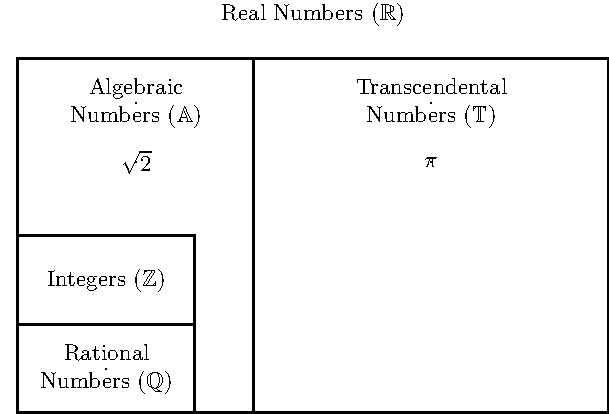
\includegraphics[width=10cm]{images/number_types.pdf}
\end{center}
\end{figure}

Note how all of these numbers are contained in the set of real numbers $\mathbb{R}$.  The real numbers thus includes both integers and rational numbers, such as $42$ and $\frac{1}{3}$, and transcendental numbers, such as $\pi$ and irrational algebraic numbers such as $\sqrt{2}$. Informally we may think of real numbers as any number with or without a decimal point that may contain an infinite decimal tail that continue in some way.
%%  CAPSULE
\begin{framed}
\textbf{Constructible Numbers}\\ A number is said to be constructible if it can be represented by a finite number of additions, subtractions, multiplications, divisions, and square root extractions of integers. Such numbers correspond to line segments which can be constructed by beginning with a unit length (that is, a length to represent the number "$1$") and keep track of what  other lengths we can produce by straightedge and compass construction.

\myindent It turns out that the totality of all possible constructible lengths, while vast, does not include every real number; as it can be shown that all constructible numbers are algebraic it follows that no transcendental numbers can be constructed. However integers such as $1,2,3$ and rationales such as $1/2, 1/3, 1/4$ and square roots, like $\sqrt{2}$ and $\sqrt{5}$ can all be constructed. Further, if we can construct two  magnitudes, we can construct their sums, difference, product and quotient and thus even complex expressions such as
\[
\sqrt{\frac{2+\frac{1}{13}\sqrt{3}}{1 + \sqrt{4 + \sqrt{3}}}}
\]
are actually constructible.
\end{framed}

Now that we have tasted the various flavors of numbers, let us return to theory of numbers and the exciting concept of divisibility.



%% DIVISIBILITY 
\section{Divisibility}
The integer $n$ is divisible by $m$ if the ratio $n/m$ is an integer. Hence we write $m|n$ when $m$ divides $n$ evenly and define
\begin{equation}\label{divisibility}
m|n \Longleftrightarrow m > 0 \textnormal{ and } n = mk \textnormal{ for some integer } k
\end{equation}

How do we know if a number is divisible by some other number ?. Here we are out of luck, in general we can only answer
this by doing full division and checking if the remainder is zero. Mathematics contains many functions that are easy to
do (such as multiplication and differentiation) but hard to undo (such as division and integration). Later on we will
see that exactly this property of division can be used to craft a simple scheme for secure communication. For now
let us consider what properties we can extract from the above definition of divisibility.
\begin{prop}
If $a > b$ and $n$ divides $a$ and $b$ evenly then it also divide their difference.
\end{prop}
\begin{proof} 
By \ref{divisibility} we have $a = nx$ and  $b = ny$ for some integral value of $x$ and $y$. Thus $a-b = nx - ny =
n(x-y)$ as desired.\qed
\end{proof}

As remarked on page \pageref{remainder} not all numbers divides evenly: 
\begin{prop}\label{division_algorithm}
If $a$ and $b$ are integers with $b\neq0$, then there is a unique pair of integers $q$ and $r$ such that
\[
a = qb+r \textnormal{ and } 0 \leq r \leq |b| 
\]
\end{prop}
Note that 
\[
\frac{a}{b} = q + \frac{r}{b}  
\] 
where for $b>0$ we have $0 \leq \frac{r}{b} < 1$ and for $b<0$ we have $0 \geq \frac{r}{b} > -1$. As example the
division $9/4$ with $a=9$ and $b=4$ becomes $9=2\cdot4 + 1$ giving us the quotient $q=2$ and remainder $r=1$
\begin{proof}
Our job is to prove that the numbers $q$ and $r$ exists, known as existence and that they are unique, also known
as uniqueness. First we prove existence. Let
\[
S = \{a-nb|n \in \mathbb{Z}\} = {a,a \pm b,a \pm 2b,...}
\]
\qed
\end{proof}

\subsection{Euclid's Algorithm}
Euclid devised a cleaver algorithm for locating the greatest common divisor. 



%% PRIMES
\section{Primes}
The \textit{prime numbers} or \textit{primes} are the numbers
\[2,3 , 5, 7, 11, 13, 17, 19, 23, 29, 31, 37 ...\]
which cannot be resolved into smaller factors\endnote{There are technical reasons for not counting 1 as a prime}. The primes are the material out of which
all numbers are build up by multiplication: thus $666 = 2 \cdot 3 \cdot 3 \cdot 37$, indeed the following holds true:

\begin{prop}\label{prim_div}
Every integer n $>$ 1 is divisible by atleast one prime
\end{prop}
\begin{proof} 
Let $A$ be a composite number (i.e. non prime). By defenition there must be some smaller number $B$ dividing evenly into $A$, where 1 $<$
$B < A$. Now either $B$ is prime or it is not. If $B$ is prime, then the original number $A$ indeed has a prime divisor, as claimed. Otherwise, $B$ is not
prime and so has a divisor, say $C$, with $1 < C < B <$ A. If $C$ is prime, we are done, for $C$ divides evenly into $B$, and $B$ divides evenly into $A$.
If $C$ is composite then it must have a propper divisor, $D$, and thus we continusly arrive at:
\[
A > B > C > D > ... > 1
\]
But all of these are positive integers, so we must reach a point in which we find a prime. Therefor any number, which is not prime itself, is divisible
by at least one prime (usually, of cause, by several).
\end{proof}

If one surveys the list of the first 50 primes
\begin{lstlisting}
2, 3, 5, 7, 11, 13, 17, 19, 23, 29, 31, 37, 41, 43, 47, 53, 59, 61, 
67, 71, 73, 79, 83, 89, 97, 101, 103, 107, 109, 113, 127, 131, 137, 
139, 149, 151, 157, 163, 167, 173, 179, 181, 191, 193, 197, 199, 
211, 223, 227, 229
\end{lstlisting}

then apparently the primes seams to be getting scarcer as the numbers go larger. Indeed between the numbers $1$ and $1000$ there are $168$ primes, whereas between $9000$ and $10.000$ there is but $112$. At first this seams logical enough since small numbers only have few possible factors and thus higher likelihood of being primes, yet one cannot help ask if we will ever reach such large numbers that the primes may eventually run out completely, rendering all subsequent numbers composite. Luckily this question had already been answered by the great greek mathematician Euclid who 300 B.C. in his IX book as proposition 20 (IX.20) indeed claimed:

\begin{prop}
Prime numbers are more than any assigned multitude of prime numbers.
\end{prop}
Euclid's terminology seams somewhat strange, what he is really proposing is that the sequence of primes does not end.
\begin{proof}
Let us for sake of eventual contradiction suppose that there is only a finite number of primes and that
\[
2, 3, 5, ..., P
\]
is the complete series (so that $P$ is the largest prime); and let us, on this hypothesis, consider the number $Q$ defined by the formula
\[
Q = (2 \cdot 3 \cdot 5 \cdots P) + 1
\]
It is plain that $Q$ is not divisible by any of $2, 3, 5, ..., P$; for it leaves the remainder $1$ when divided by any one of these numbers. But, if $Q$ is not  prime, then by \ref{prim_div} it is divisible by some prime, and therefore there is a prime (which may be $Q$ itself) greater than any of them. This contradicts our hypothesis, that there is no prime greater than $P$; and therefore this hypothesis is false.
\end{proof}

Finding and counting the primes is a long standing hobby for mathematicians, and one might ask if it can be automated. One such method was discovered by the greek mathematician Eratosthenes (ca. 284-192 B.C.) who as the chief librarian at the great Library at Alexandria spend much of  his time studying mathematics, astronomy and philosophy. His method (known as Eratosthenes sieve) is as follows; write a list of all the consecutive integers, starting with $2$, among which you want to find the primes. As $2$ is prime, cross all subsequent multiples off. The next integer that has not yet been crossed of (3) must then also be prime and so we can eliminate all of its multiples. As we continue in this manner we will clearly sieve out all composite numbers and be left with the primes.
\begin{verse}\emph{
Sift the Twos and sift the Threes,\\
The Sieve of Eratosthenes.\\
When the multiples sublime,\\
The numbers that remain are Prime.}
\end{verse}
although this method will indeed generate the primes, it is not as efficient as one might have liked (although optimized and more complex methods exists). Later we shall encounter the prime counting function $\pi(n)$,  which outputs the number of primes less than or equal to a given number $n$ (the use of $\pi$ in this function is an unfortunate standard as it has nothing to do with the constant $3.1415...$).


\section{Fermat's Little Theorem}


%% EXERCISES
\newpage
\section*{Exercises}
\addcontentsline{toc}{section}{Exercises} 
\subsection*{Warmups}
% 1
\begin{exc}\label{ex:elem-num:1}
In 2000 the Jordanian mathematician, Murad A. AlDamen\endnote{Found on the prime puzzlers project, at: \emph{http://www.primepuzzles.net/puzzles/puzz\_101.htm}} devised the following method for testing divisibility
\begin{enumerate}
\item Use Murad's method to answer the following: does $61$ divides $3598207$ ?
\item Prove Murad's method.
\end{enumerate}
\end{exc}

%% ENDNOTES
\theendnotes

%% FROM Mathematics
Numbers that can be obtained by raising 2 to a power and then subtracting 1 are called Mersenne numbers, for reasons I’ll give later in the chapter. Prime numbers of this particular form are called Mersenne primes 

fundamental theorem of arithmetic: that every natural number greater than 1 is either prime, or else can be expressed as a product of primes in a way which is unique except for the order in which the primes are arranged.

the prime numbers are the basic building blocks from which all the natural numbers are constructed.

%% TODO
%% Of particular interest in the non-negative integers i.e. elements of the set $\{0,1,2,3...\}}$, also known as the natural numbers and usually abbreviate as $\N$.
%% - Fermat capsule (and his claims)
%% - Euler capsule (and his teachers)
%% - phi and e are irrational
%% - prime counting function
%% - eliptic curves
%% - enhanced prime finding and locating algorihms (sqare root of n}
%% - one way functions and cryptography (RSA - the code book)
